% \documentclass{standalone}
% \usepackage{tikz}
% \usetikzlibrary{patterns}
% \begin{document}
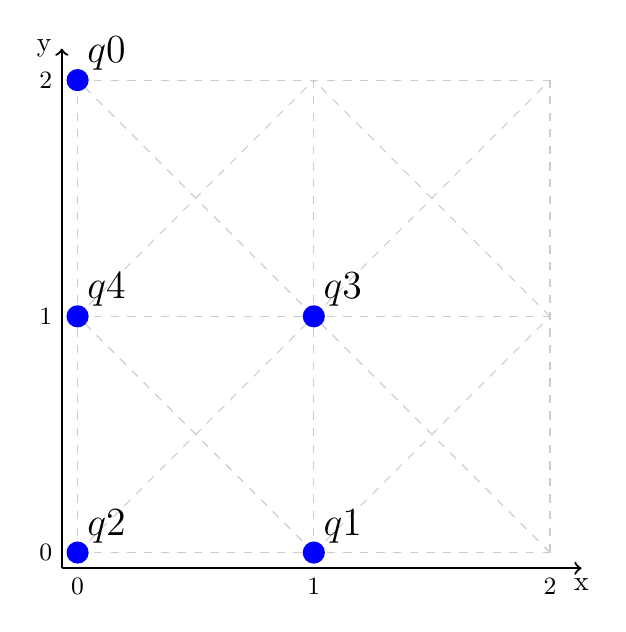
\begin{tikzpicture}
    \definecolor{lightgray}{rgb}{0.8,0.8,0.8}
    \definecolor{darkgreen}{rgb}{0  ,0.5,0  }
    \tikzset{
        unuseNode/.style={
            circle,
            draw=blue,
            dashed, % Dashed outline
            % fill=red, % Solid fill color
            % pattern=vertical lines, % Pattern type
            minimum size=8pt,
            inner sep=0pt
        },
        useNode/.style={circle, draw=none, fill=blue,minimum size=8pt, inner sep=0pt},
        fontNode1/.style={above right, font=\Large },
        fontNode2/.style={right, midway,font=\small}
    }
    % Set the color and style of the grid lines
    \draw[lightgray, dashed, xstep =3, ystep =3] (0,0) grid (6,6);
    
    % Draw the x and y axis arrows
    \draw[->, thick] (-0.2,-0.2) -- (6.4,-0.2) node[below] {x};
    \draw[->, thick] (-0.2,-0.2) -- (-0.2,6.4) node[left] {y};

    % Draw the bevels (diagonals in each grid square)
    \foreach \x in {0,3} {
        \foreach \y in {0,3} {
            \draw[lightgray, dashed] (\x,\y) -- (\x+3,\y+3); % Diagonal from bottom-left to top-right
            \draw[lightgray, dashed] (\x+3,\y) -- (\x,\y+3); % Diagonal from bottom-right to top-left
        }
    }
    
    % Add labels for the x-axis
    \foreach \x in {0,1,2} {
        \node[below] at ({3*\x}, -0.2) {\small \x};
    }

    % Add labels for the y-axis
    \foreach \y in {0,1,2} {
        \node[left] at (-0.2, {3*\y}) {\small \y};
    }

    \node[useNode] (q0) at (0,6) {};
    \node[fontNode1] at (q0) {$q0$};
    \node[useNode] (q1) at (3,0) {};
    \node[fontNode1] at (q1) {$q1$};
    \node[useNode] (q2) at (0,0) {};
    \node[fontNode1] at (q2) {$q2$};
    \node[useNode] (q3) at (3,3) {};
    \node[fontNode1] at (q3) {$q3$};
    \node[useNode] (q4) at (0,3) {};
    \node[fontNode1] at (q4) {$q4$};
\end{tikzpicture}
% \end{document}
